\chapter{数据更新}
数据更新工作在深圳市交通仿真系统(二期) 已有的\ppyear 年静态 GIS 数据
和动态交通数据基础上,根据 \pyear 年各类数据变化情况对底层数据进行更新,
将系统的输入数据时间更新至 \pyear 年。

数据更新工作是后续数据挖掘、数据查询系统更新以及模型系统更新的前提,
是一项重要的基础性工作。

\section{动态交通数据处理}
动态交通数据指的是带有时间信息的交通数据, 可以通过数据本身来反映不
同时段交通的特征以及变化趋势。 其更新频率高,通常 1 分钟就会更新 2-5 次,
可以反映交通的实时状态和动态变化,因此称为动态数据。

深圳市交通仿真系统(二期)中囊括的动态交通数据包括出租车 GPS 数据、
公交车 GPS 数据、深圳通 IC 刷卡数据 (轨道和常规公交)、车牌识别数据四大类。
本项目的目标就是,将这四类数据从原始状态开始经过一系列技术加工, 最终更
新至符合深圳市交通仿真系统(二期)输入格式的标准化数据。

\subsection{原始数据采集}
动态交通数据来源于不同的单位,因此数据采集工作就是按照一定的时间周
期从这些单位获取到最新的原始数据。

本项目按季度分别从市交委、市交警局监控中心、东部公交公司、西部公交
公司、 巴士集团公司、 深圳通公司、地铁 ACC 公司通过现场拷贝、网络传输和光
盘邮寄几种方式获取所需数据。 本项目已采集的原始动态数据至 \pyear 年 12 月。

\smalltitle{公交刷卡数据}
\begin{longtabu} to \textwidth {|c|X[1,l]|}
\hline
数据内容 & 包括每日350万次公交刷卡的线路、站点、时间、车牌以及卡号等信息\\\hline
数据大小 & \pyear 年全年数据大小约 14GB\\\hline
数据格式 & ASCII 文本格式\\\hline
数据来源 & 深圳通公司\\\hline
采集方式 & 每季度由深圳通公司将当季度数据刻录光盘, 再派指定人员取回\\
\hline
\end{longtabu}
\addtocounter{table}{-1} % 不需要计数

\smalltitle{轨道刷卡数据}
\begin{table}[ht]
\centering
\begin{tabularx}{\textwidth}{|c|X|}
\hline
数据内容 & 包括轨道刷卡和投币每日650万次的进出站点、时间和卡号信息\\\hline
数据大小 & \pyear 年全年数据大小约 15GB\\\hline
数据格式 & ASCII 文本格式\\\hline
数据来源 & 地铁ACC公司\\\hline
采集方式 & 每季度由 ACC 公司将当季度数据刻录光盘, 再派指定人员取回\\
\hline
\end{tabularx}
\end{table}

\smalltitle{车牌识别数据}
\begin{table}[ht]
\centering
\begin{tabularx}{\textwidth}{|c|X|}
\hline
数据内容 & 包括全市视频监测点和车牌识别系统提供的车牌识别数据\\\hline
数据大小 & \pyear 年全年数据大小约480GB\\\hline
数据格式 & ASCII 文本格式\\\hline
数据来源 & 市交警监控中心\\\hline
采集方式 & 每季度派指定人员去市交警监控中心现场拷贝\\
\hline
\end{tabularx}
\end{table}

\smalltitle{公交 GPS 数据}
\begin{table}[ht]
\centering
\begin{tabularx}{\textwidth}{|c|X|}
\hline
数据内容 & 包括按每 10 秒/回传频率的出租车运行 GPS 数据\\\hline
数据大小 & \pyear 年全年数据大小约 350GB\\\hline
数据格式 & ASCII 文本格式\\\hline
数据来源 & 市交委\\\hline
采集方式 & 每季度由专人去现场拷贝\\
\hline
\end{tabularx}
\end{table}

\subsection{数据预处理}
由于原始数据来源于不同的单位,原始数据的格式存在很大的差异,为达到
能够统一输入深圳市交通仿真系统(二期) 数据平台的要求, 需要按照原系统设
计的表格结构对数据进行字段顺序调整、精简和合并等预处理工作实现标准化,
本项目中针对每类数据的特点,开发了专门的程序进行处理,实现了自动化作业。
\tref{tbl:数据预处理工作}是每类数据处理的工作内容。

\begin{table}[ht]\centering
  \caption{数据预处理工作\label{tbl:数据预处理工作}} 
  \begin{tabularx}{\textwidth}{|c|X|}
    \hline
    {\bfseries 数据类型} & \multicolumn{1}{c|}{\bfseries{预处理工作}}\\\hline
     公交刷卡数据 & 清理无效字符;按照系统表结构调整顺序\\\hline
     轨道刷卡数据 & 清理无效字符;按照系统表结构调整顺序\\\hline
     车牌识别数据 & 清理无效字符;合并成每天一个文件;按照系统表结构调整顺序\\\hline
     公交GPS数据 & 清理无效字符和错误数据;合并成每天一个文件;按照系统表结构调整顺序\\
    \hline
  \end{tabularx}
\end{table}
% 另外,为了后续计算道路车速、 公交车车速、 出租车 OD 和空重车等指标,
% 需要对出租车数据和公交 GPS 数据进行进一步的预标准化预处理, 所有的工作
% 都由专门开发的程序来自动化完成。

% \smalltitle{出租车 GPS 数据标准化}
% 预处理程序为 FCD\_SyncData-SZ,主要包括: 程序运行库、批处理程序
% statnew.bat 和配置文件 config.xml。操作步骤如下:

% \begin{nbeae}
% \item 设置输入文件路径\\
% \indenttext{建立两个文件夹,用于存放 GPS 原始数据和标准化后的 GPS 数据。例如,
% 在 E 盘根目录下建立文件夹“GPSINPUT”,“GPSOUTPUT”。将 GPS 原始数据
% 解压后放入“ GPSINPUT”下,文件放置规则需按照年月日顺序依次建立相应文
% 件夹,然后放入。如:\pyear 年 1 月 1 日数据,放置路径为
% “E:$\backslash$GPSINPUT$\backslash$\pyear$\backslash$1$\backslash$1$\backslash$”,
% \pyear 年 1 月 2 日数据,放置路径为“E:$\backslash$GPSINPUT$\backslash$\pyear
% $\backslash$1$\backslash$2$\backslash$”,其余数据依次类
% 推,将需标准化的 GPS 数据按照该规则放置到正确路径下即可。}
% \item 设置配置文件\\
% \indenttext{将 GPS 输入路径与输出路径写入系统配置文件“ config.xml”中。将配置文
% 件中如下部分正确填写即可。}\\
% \indenttext{<frompath> E://GPSINPUT//</frompath>}\\
% \indenttext{<topath> E://GPSOUTPUT//</topath>}\\
% \indenttext{Frompath 和 topath 标签中间的路径为需要填写的输入和输出文件路径。 路
% 径只需配置到“年”的上一级路径即可,如上示例中,“ 2015”文件夹上一级为
% “ GPSINPUT”,那么“ frompath”只需要配置为“ E://GPSINPUT//”即可。}
% \end{nbeae}

\subsection{分类集中存储}
预处理后的动态交通数据将通过 FTP 方式上传到数据挖掘主机(配置见附
录), 按照预先设定的分类目录进行集中存储,作为后续数据挖掘的输入。

预处理动态交通数据每季度上传一次,包含三个月,每月一周(周一至周日
7 天)的数据。在数据挖掘主机中,建立了以下原始数据目录结构,用于存放这
些数据。\fref{tbl:数据挖掘主机中分类集中存储文件的目录结构}是存储文件的目录结构。

\begin{table}[!ht]\centering
  \caption{数据挖掘主机中分类集中存储文件的目录结构\label{tbl:数据挖掘主机中分类集中存储文件的目录结构}} 
  \begin{tabularx}{\textwidth}{|Y|Y|Y|Y|Y|}
    \hline
    \multicolumn{1}{|c|}{\bfseries 根目录} & \multicolumn{1}{c|}{\bfseries 二级目录} & 
    \multicolumn{1}{c|}{\bfseries 三级目录} & \multicolumn{1}{c|}{\bfseries 四级目录} &
    \multicolumn{1}{c|}{}\\\hline
    \$DM\_HOME & 年份 & 季度 & 数据类型 & 文件\\
    \hline
  \end{tabularx}
\end{table}

其 中 , \$DM\_HOME 指 数 据 挖 掘 主 机 存 放 数 据 的 根 目 录 , 默 认 为
/home/dm/data。在根目录下, 每年数据存放在名称为“ 4 位年份”的二级目录中,
例如 2013、 2014、 2015。二级目录下创建四个三级目录,目录名称为: s+季度
( 1-4), 该子目录用于存放某年一个季度的数据。在三季目录下,按不同种类的
交通数据分别建立对应的四级目录:

\begin{para}
\item[目录 ic] 存储 IC 刷卡数据(包括轨道和巴士刷卡数据)
\item[目录 gps] 存储巴士 GPS 数据
\item[目录 lp] 存储车牌识别数据
\end{para}

在四级目录下, 按照每天一个文件的形式存放相应的数据文件。 如果原始数
据以压缩文件方式提供,在写入对应目录之间,必须先进行解压缩处理,然后才
写入目录。\fref{fig:分类集中存储后的目录结构}为分类集中存储后的目录结构截图。

\clearpage
\begin{figure}[!ht]
  \centering
%\begin{center}
  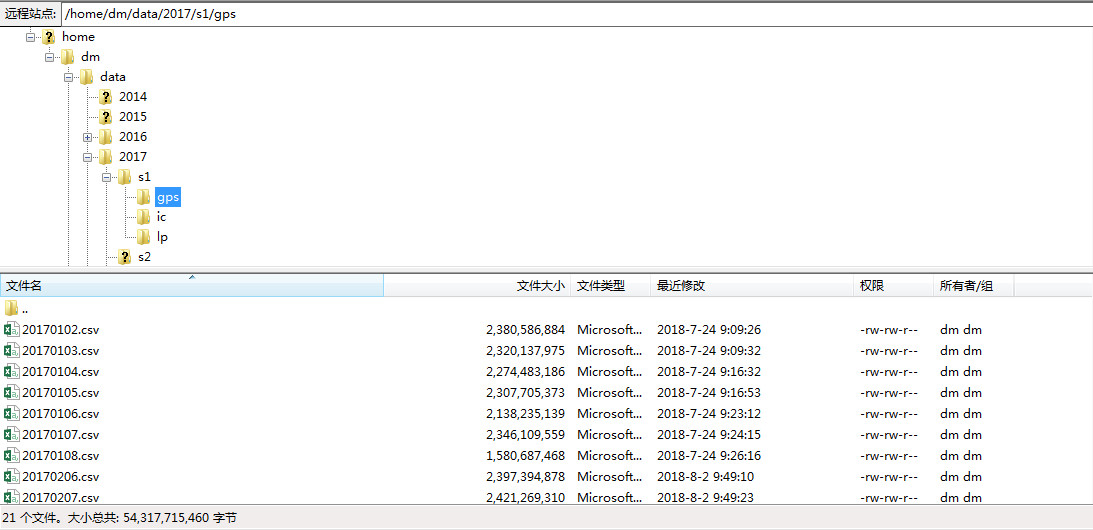
\includegraphics[width=\textwidth]{figures/chp02_分类集中存储后的目录结构.jpg}
  \caption{分类集中存储后的目录结构\label{fig:分类集中存储后的目录结构}} 
%\end{center}   
\end{figure}

\section{静态 GIS 数据处理}
静态 GIS 数据指用于展示和分析的 GIS 图层数据, 包括各类区域边界、 道
路网络、公交网络站点的形状和属性信息等, 主要用于制作各类交通专题图、基
础统计以及辅助数据挖掘计算。 其变化频率低、 更新周期较长,一般为一年更新
一次,因此相对于动态交通数据的高更新频率来说属于静态数据。

\subsection{现有静态 GIS 数据}
深圳市交通仿真系统(二期) 中囊括的静态 GIS 数据包括: 基础 GIS 数据
(行政区、水系、绿地、法定图则、组团、街道),基层路网数据(道路节点、
路段、交通小区、主要节点数据),公交和轨道 GIS 数据(公交站点、公交网络、
轨道站点、轨道网络),调查数据(居民出行调查、轨道二期开通后调查、交叉
口/断面流量调查等),现状和规划土地利用(建筑物普查数据、规划一张图),
现状和规划人口岗位数据, POI 数据(医院、学校、口岸、火车站、飞机场、港
口、公共停车场、 检测器), 共 4 大类 26 小类。详细表信息见附表。

其中, 道路数据和公交数据涉及后续的数据挖掘系统输入,需要进行年度更
新,其他 GIS 数据根据需求不定期进行更新。 为了提高工作效率, 数据更新工
作按照不同 GIS 图层并行开展, 更新后的 GIS 数据以 shapefile 格式进行存储,
待后续数据挖掘和数据查询系统使用。


% \begin{longtabu} to \textwidth {|X[1,c]|X[1,c]|X[1,c]|X[1.2,c]|X[1.2,c]|}
% \caption{现有静态 GIS 数据\label{tbl:现有静态 GIS 数据}} 
%   \hline
%   \multicolumn{1}{|c|}{\bfseries 类别} & \multicolumn{1}{c|}{\bfseries 名称} &
%   \multicolumn{1}{c|}{\bfseries 格式} & \multicolumn{1}{c|}{\bfseries 主要属性} &
%   \multicolumn{1}{c|}{\bfseries 更新周期} \\\hline
%    & 行政区 & shapefile & 名称、 关内关外 & 由信息中心提供\\\hline
%   \multirow{6}*{基础GIS数据} & 水系 & shapefile & 名称 & 由信息中心提供\\\cline{2-5}
%    & 绿地 & shapefile & 名称 & 由信息中心提供\\\cline{2-5}
%    & 法定图则 & shapefile & 名称 & 由信息中心提供\\\cline{2-5}
%    & 组团 & shapefile & 名称 & 由信息中心提供\\\cline{2-5}
%    & 街道 & shapefile & 名称 & 由信息中心提供\\\cline{2-5}
%    & 人口普查小区 & shapefile & 名称 & 由信息中心提供\\\hline
%    \multirow{5}*{基础路网数据} & 现状道路节点 & shapefile & 坐标、节点类型、所在行政区、所在交通小区、所在街
% 道、所在组团、所在法定图则、交叉口控制类型、立交类型 & 由信息中心提供\\\cline{2-5}
%    & 主要交叉口 & shapefile & 同上 & 不定期  \\\cline{2-5}
%    & 现状道路网络 & shapefile & 起止节点编号、起止道路名称、道路
% 名称、车道数、长度、宽度、机动车道宽度、非机动车道宽度、人行道宽度、 机非分隔带宽
% 度、 中央分隔带宽度、 红线宽度、 道路等级、行车方向、建设方式、 分割类型、 是否具备公交
% 专用道、 交通系统集、 设计车速、 路段通行能力、 路段延误函数、 所在行政区、 所在交通小
% 区、 所在街道、 所在组团、 所在法定图则、 最后更新时间 & 年度 \\\cline{2-5}
%    & 规划道路网络 & shapefile & 同上 & 不定期 \\\cline{2-5}
%    & 交通小区 & shapefile & 形心坐标、所在行政区、所在街道、所在组团、所在法定图则 & 不定期\\\cline{2-5}
% \hline
% \end{longtabu}

